%! TEX root = ../thesis.tex

\chapter{Physics of cosmic rays}
\label{chap:physical-background}

The term cosmic ray is used in the context of particles that travel through space close to the speed of light. Their kinetic energy far exceeds their rest mass, 
and ranges from $\mathcal{O}(\SI{}{\giga\electronvolt})$ for solar particles to energies exceeding $10^{20}$\SI{}{\electronvolt} for atoms of extragalactic origin. 
The latter are typically referred to as \textbf{U}ltra \textbf{H}igh \textbf{E}nergy CRs (UHECRs) in literature.

This chapter aims to introduce the general physical principles needed to describe cosmic rays. For this purpose, an overview of the origin of CRs is presented in
\autoref{sec:cr-acceleration}, discussions regarding their propagation in space, the resulting primary and energy composition are given in 
\autoref{sec:cr-propagation}, \autoref{sec:cr-composition} and \autoref{sec:cr-energy-spectrum} respectively. Immediately following is a summary of the discovery of cosmic rays in \autoref{sec:cr-history}.

\section{History}
\label{sec:cr-history}

A first hint at the existance of high-energy particles in the upper atmosphere was given by Hess in 1912, who found that the discharge rate of an electroscope is 
altitude-dependant. Millikan coined the term cosmic "rays" for these particles, as he argued the ionizing radiation must be part of the electromagnetic spectrum 
\cite{millikan1928origin}. This was later, at least partially, falsified with the discovery of the east-west effect \cite{johnson1938note}. Hess' observation 
however withstood the tests of time and was ultimately recognized with the Nobel prize in physics in 1936 \cite{nobelprize1936}. Two years later, in 1938, Pierre 
Auger showed via coincidence measurements that cosmic rays in fact originate from outer space, and gave a first description of extensive air showers 
\cite{auger1939extensive}. Another 60 years later, the Pierre Auger collaboration would adopt his experimental setup and name in their search for cosmic rays of 
the highest energies.

In the meantime, numerous results from different cosmic ray detectors all over the globe have helped propel the related fields of particle physics, astro physics 
and cosmology to new insights. Observations from cosmic ray physics serve as a valuable cross-check to the hadronic interaction models developed e.g. at CERN 
\cite{ostapchenko2007status}. New theories modeling the final moments in the life of stars have arisen thanks to results from e.g. Kamiokande 
\cite{goldman1988implications}. Last but not least, publications by the Pierre Auger collaboration regarding the CR energy spectrum and flux help refine knowledge of 
our cosmic neighbourhood \cite{abraham2010measurement, aab2015searches}.

\section{Acceleration}
\label{sec:cr-acceleration}

Following the detection of a cosmic ray on earth, the logically following questions are "where did it originate from?", and "how was it accelerated?". It is clear 
that particles with extreme energies must be created under extreme conditions. In particular regions with large \textbf{e}lectro\textbf{m}agnetic (EM) fields, either 
in field strength or spatial extent, play a big role in the acceleration of CRs for reasons listed in the following pages. Several acceleration mechanisms have been identified.

\subsection{Diffusive shock acceleration (Fermi I)}
\label{ssec:cr-fermi-i}

\textbf{S}uper \textbf{N}ova \textbf{R}emnants (SNR) typically feature a plasma sphere propagating outwards from the former stars core into the 
\textbf{I}nter \textbf{S}tellar \textbf{M}edium (ISM), in this region of plasma any magnetic field lines will be comoving, according to Alfvén's theorem 
\cite{alfven1942existence}. First realised by Fermi, such SNR shock fronts serve as source of high-energy CRs \cite{fermi1949origin}.

If a low-energy particle is injected into the SNR shock front, it will eventually be reflected by the local $\vec{B}$-field. If the diffusion length within the
plasma is much smaller than the spatial extent of the SNR, the shock front can be modelled as a plane, and the process is analogous to an elastic reflection 
against a wall. Consequently, if $\frac{\text{d}\vec{B}}{\text{d}t} = 0$, this does not cause the particle to gain any energy, espically because 
$W = \vec{F}_\text{L} \cdot \vec{r} \propto (\vec{v}\times\vec{B})\,\cdot\,\vec{r} = 0$. However, because the $\vec{B}$-field is moving radially outward alongside 
the plasma, a net energy gain of 

\begin{equation}
\label{eq:fermi-energy-gain}
\Delta E = +\beta_\text{SNR} \cdot E_0
\end{equation}

arises, where $\beta_\text{SNR} = |\vec{v}_\text{SNR}|\,/\,c$ and $E_0$ are the velocity of the shock-front and the initial energy of the particle. From chapter 7 
in \cite{fermi1949origin} it follows that ionization losses within the shock front are not completely negligible. Hence a particle must have a sufficient energy 
such that $\Delta E$ in \autoref{eq:fermi-energy-gain} exceeds possible ionization losses. The corresponding threshold for the primary energy above which 
acceleration occurs is dubbed the injection energy, and is of the order of \SI{200}{\mega\electronvolt} for protons. 

Furthermore, because typically $\beta_\text{SNR} \leq 0.10$ a single acceleration cycle is not enough to explain the CR energies observed on earth. Instead, 
multiple cycles are needed. This requires additional, focusing $\vec{B}$-fields, provided for example by the ISM, which alter the trajectory of injected particles 
such that they can be reflected off the shock-front again.

With each cycle, the particles rigidity $R = |\vec{p}|c\,/\,q$ increases, until its gyroradius $\rho = R / |\vec{B}|$ exceeds the spatial extent of the focusing 
$\vec{B}$-field and the particle escapes into space. With an effective ejection probability $p$ per cycle, the energy after $n$ cycles and the expected flux w.r.t
energy, $\Upphi(E)$, becomes roughly

\begin{equation}
\label{eq:fermi-energy}
E(n) = E_0\;\left( 1 + \beta_\text{SNR} \right)^n.
\end{equation}

\begin{align*}
                                                        N(n) &= N_0 \;\left( 1 - p \right)^n \\
\Leftrightarrow\;\;\;\;\,\log\left( \frac{N(n)}{N_0} \right) &= n\cdot\log\left( 1-p \right) \\ 
\Leftrightarrow\qquad\qquad\qquad\;\;&\stackrel{\mathmakebox[\widthof{=}]{\eqref{eq:fermi-energy}}}{=}\;\log\left( \frac{E(n)}{E_0} \right) 
\frac{\log(1-p)}{\log(1+\beta_\text{SNR})} \\
\Leftrightarrow\qquad\qquad                             N(E) &= N_0\cdot\left( \frac{E(n)}{E_0} \right)^{\log(1 - p)\;/\;\log(1 + \beta_\text{SNR})} \\
\Rightarrow \qquad\qquad                           \Upphi(E) &= \frac{ \text{d}N }{ \text{d}E } \propto E(n)^{\alpha - 1}, \numberthis\label{eq:fermi-spectrum}
\end{align*}

where $\alpha = \frac{\log(1 - p)}{\log(1 + \beta_\text{SNR})}$ in \autoref{eq:fermi-spectrum} is a spectral coefficient whose exact value will depend on the age 
of the SNR ($\beta_\text{SNR}$ decreases with age), the injected particle (different primaries have different injection energies and ejection probabilities), as 
well as many other factors that are often not known a priori. It can however be observed that the expected spectrum is a power law in the ranges from injection energy 
to a cutoff at the highest energies, which arises due to the finite lifetime of SNRs.

Results from several studies (e.g. \cite{aab2015searches, hillas2005can, blasi2013origin}) hint that the presented first order Fermi acceleration mechanism is the 
main source of galactic CRs, extrasolar particles that originate from within the milky way, with energies ranging up to orders 
$\mathcal{O}(\SI{}{\tera\electronvolt})$.

\subsection{Stochastic scattering acceleration (Fermi II)}
\label{ssec:cr-fermi-ii}

Second order (or stochastic) Fermi acceleration is the more general case of \autoref{ssec:cr-fermi-i} and represents the original idea developed by Fermi in 
\cite{fermi1949origin}. The underlaying principle of scattering particles off plasma clouds remains unchanged. However, if the diffusion length within the cloud 
exceeds its radius of curvature, the energy gain per collision instead becomes

\begin{equation}
\Delta E \propto + \left( \beta_\text{SNR}\right)^2 \cdot E_0.
\end{equation}

Logically, this represents a much more inefficient acceleration mechanism, but is nevertheless observed in nature under certain circumstances (c.f. 
\cite{asano2015most}).

\subsection{Centrifugal acceleration in rotating $\vec{B}$-fields}
\label{ssec:cr-centrifugal-acceleration}

Some astrophysical objects such as pulsars or \textbf{A}ctive \textbf{G}alactic \textbf{N}uclei (AGNs) possess strong magnetic fields ranging from \SI{1}{\tesla}
for some AGNs \cite{daly2019black} to $\approx\SI{10}{\giga\tesla}$ for magnetars, a subset of pulsars with extremely high magnetic flux densities 
\cite{flowers1977evolution}.

If such objects rotate at an angular velocity $\Omega$, which is in general nonzero, charged particles at a radial distance $r$ from the rotation axis will undergo
centrifugal acceleration. In particular, their Lorentz factor $\gamma$ behaves like \autoref{eq:lorentz-factor-acceleration} \cite{rieger1999particle}.

\begin{equation}
\label{eq:lorentz-factor-acceleration}
\gamma := \frac{E}{m_0 c^2} = \frac{\gamma_0}{1 - \left(\frac{\Omega r}{c}\right)^2},
\end{equation}

where $m_0$ is the rest mass of the particle and $\gamma_0$ the prior Lorentz factor before acceleration. It follows that a test particle can in theory gain an
arbitrarily high energy from this process by outspiraling towards the light cylinder surface, where $\Omega\cdot r = c$. In reality however, these processes are
stopped by e.g. inverse Compton scattering at some point \cite{osmanov2007efficiency}. In any case, \cite{rieger1999particle} and \cite{osmanov2007efficiency}
conclude that values of $\gamma \approx 10^7-10^8$ are possible, corresponding to protons at $\approx\SI{10}{\peta\electronvolt}-\SI{10}{\peta\electronvolt}$ or 
iron nuclei at $\approx\SI{500}{\peta\electronvolt}-\SI{5}{\exa\electronvolt}$ energy.

\subsection{Direct electrostatic acceleration}
\label{ssec:cr-electrostatic-acceleration}

The presence of non-static $\vec{B}$-fields implies the existance of (in vacuum) comparably strong $\vec{E}$-fields and a corresponding electrical potential 
difference $\Upphi$ across different regions within the magnetosphere. A back-of-the-envelope calculation reveals that they are (neglecting constant factors) 
proportional to

\begin{align}
|\vec{E}| &\propto \frac{\Omega\;r_0}{c} \cdot |\vec{B}|, \\
\Upphi &\propto r_0 \cdot |\vec{E}|,
\end{align}

where $r_0$ is the radius of the central object rotating at an angular frequency $\Omega$. Consequently, an ion with atomic number $Z$ can be accelerated to 
energies $E = Z \cdot e \cdot \Upphi$, which can in some cases easily exceed $10^{20}\SI{}{\electronvolt}$ \cite{rieger2009cosmic}. 

Some caveats to this consideration need to be mentioned. Screening effects from plasma clouds surrounding the central body are expected to limit the electrical 
field strength, and maximum acceleration energy by extension. Additionally, losses via e.g. Bremsstrahlung have been neglected in the above calculation, limiting
the maximum attainable energy in theory even further. 

\subsection{Other types \& general classification}
\label{ssec:cr-hillas-plot}

Several acceleration mechanisms have been discussed. A plethora of other interactions that are able to accelerate elementary particles to fantastic energies remain
unmentioned, or even undiscovered, as CR physics is an active area of research. In general though the driving force behind all considered (and non-considered)
acceleration mechanisms are thought to be (electro-) magnetic fields, given their infinite range and large coupling strengths compared to other fundamental 
forces. Consequently, the maximum energy a specific CR accelerator with magnetic field $\vec{B}$ and size $L$ moving at velocity $\beta c$ can in theory provide 
for a particle with charge $Ze$ is given by the Hillas formula \cite{hillas1984origin}:

\begin{equation}
\label{eq:hillas-formula}
E_\text{max}\;[\SI{}{\peta\electronvolt}] = |\vec{B}|\;[\SI{}{\micro\gauss}] \cdot L\;[\SI{}{\parsec}] \cdot Z \cdot \beta
\end{equation}

This allows for an elegant classification of different cosmic ray sources, in part discussed on the previous pages, according to the Hillas plot shown in 
\autoref{fig:hillas-plot}.

\begin{figure}
	\centering
	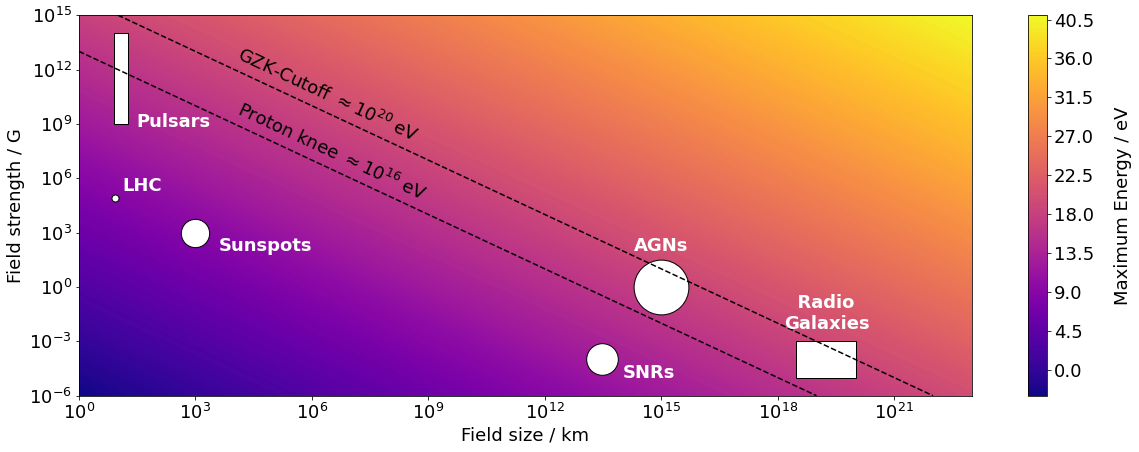
\includegraphics[width=1\textwidth]{./plots/hillas_plot.png}
	\caption{Rough estimate of field strength and size of different CR sources as well as the corresponding maximum energy estimated with 
    \autoref{eq:hillas-formula} ($\beta = Z = 1$). Isoenergetic lines mark notable points in the energy spectrum discussed in 
    \autoref{sec:cr-energy-spectrum}.}
	\label{fig:hillas-plot}
\end{figure}

\subsection{Acceleration of uncharged particles}
\label{ssec:cr-uncharged-acceleration}

Particles like neutrons, neutrinos or photons possess no electromagnetic charge $q = 0$. Assuming \autoref{eq:hillas-formula} holds in these cases, they 
should thus not appear in the CR spectrum. This is in disagreement with reality, where energies from \SI{100}{\giga\electronvolt} up to 
$\approx\SI{100}{\exa\electronvolt}$ have been observed \cite{abeysekara2018very, ishihara2016extremely}. Consequently, additional interaction channels are 
required to explain the existance of such uncharged CRs.

High energy $\gamma$-rays in particular can be created by accelerated, charged particles via Bremsstrahlung. This occurs for example during centrifugal 
acceleration near pulsars or AGNs (compare \autoref{ssec:cr-centrifugal-acceleration}). Furthermore, inverse Compton scattering with a high-energy cosmic ray can 
imply a significant energy gain for a photon \cite{jones1965inverse}.

Uncharged CRs are also frequently produced in nuclear interactions, such as e.g. deeply inelastic scattering of charged CRs with the ISM. This espically 
contributes to the CR photon spectrum, as high energy $\pi^0$ are often byproducts of such scattering processes. The uncharged pions then decay into two photons. 
Furthermore, neutrons or neutrinos can originate from interactions involving the weak force. When a proton converts to $p\rightarrow n+e^++\bar{\nu_e}$ during the 
dacy of a UHECR ion, the resulting decay products, positron, neutron and electron-antineutrino inherit the parents' energy, and are thus high energy cosmic rays as 
well.

\section{Propagation}
\label{sec:cr-propagation}

Once a cosmic ray has been observed coming from some arrival direction $(\phi, \theta)$, backtracking its' trajectory to an eventual origin is, ignoring external 
factors, in the literal sense, straight forward. It has been shown however that several effects need to be considered for an accurate treatment of CR propagation. 

For uncharged CRs ($\gamma$, $n$), this task is simple. Such particles are not deflected by cosmic $\vec{E}$ and $\vec{B}$-fields. Possible interactions either 
demand the destruction of the particle (pair production, weak decay), or occur close to the source (e.g. Compton scattering), in which case the observed arrival 
direction will still be coincident with the actual source \cite{fermi201398}. Gravitational lensing effects in some cases alter the trajectory of extragalactic 
photons. Such phenomena (if present in the first place) are however well understood in the scope of general relativity, and can be corrected for 
\cite{bartelmann2010gravitational, bartelmann2001weak}.

\subsection{Intergalactic propagation \& transport equation}
\label{ssec:transport-equation}

Contrary, charged particles ($e^\pm$, $p$, ions) propagate along non-trivial paths within galaxies due to deflections from solar- and galactic EM-fields. While the 
galactic field is coherent over large scales, numerous irregular magnetic domains, seeded in part by individual stars complicate CR propagation to essentially a 
three-dimensional random walk \cite{haverkorn2015magnetic}. It is thus challenging to pinpoint the origin of a charged cosmic ray. 

Nevertheless, related queries, such as for example the question whether or not a particle of given energy is likely to be of extragalactic origin can be answered by
examining the distribution of cosmic rays within a region of spacetime. The behaviour of a population of $n_i$ particles of type $i$ can be approximately recreated 
via the below transport equation:

\begin{equation*}
\label{eq:leaky-box-model}
\frac{\partial n_i}{\partial t} =   \underbrace{Q_i \vphantom{\left(\sum\limits_{j>i}\frac{p_{ij}}{\tau_{\text{spal.},\,j}} n_j\right)}}_\text{Source} 
 								  + \underbrace{\nabla D_i \left( \nabla n_i \right) \vphantom{\left(\sum\limits_{j>i}\frac{p_{ij}}{\tau_{\text{spal.},\,j}} n_j\right)}}_\text{Diffusion} 
								  - \underbrace{\frac{\partial k_i(E)}{\partial E} \vphantom{\left(\sum\limits_{j>i}\frac{p_{ij}}{\tau_{\text{spal.},\,j}} n_j\right)}}_\text{Energy} 
								  - \underbrace{\left( \frac{n_i}{\tau_{\text{spal.},\,i}} - \sum\limits_{j>i} \frac{n_j\,p_{ij}}{\tau_{\text{spal.},\,j}} \right)}_\text{Spallation}
								  - \underbrace{\left( \frac{n_i}{\tau_{\text{rad.},\,i}} - \sum\limits_{j>i} \frac{ n_j\,d_{ij}}{\tau_{\text{rad.},\,j}} \right)}_\text{Weak decay}
\end{equation*}

\begin{itemize}
	\item \textbf{Source} $Q_i$ :

	The source term is responsible for the creation of CR particles (of type $i$). The exact form of $Q_i$ will depend on the considered creation process. For 
	example, the near instantaneous creation of $n_\gamma$ photons in a \textbf{G}amma-\textbf{R}ay \textbf{B}urst (GRB) at time $t_0$ and location $\vec{r_0}$ can 
	be modelled like $Q_\gamma = n_\gamma \; \delta(\vec{r} - \vec{r_0}) \, \delta(t - t_0)$.

	\item \textbf{Diffusion} $\nabla D_i \left( \nabla n_i \right)$ :

	The random walk mentioned above is accounted for in the diffusion term, which takes a similar form to the Stokes-Einstein equation. The diffusion 
	coefficient(s) $D_i$ in the most general case take a tensor form due to anisotropic diffusion in different directions. Furthermore, $D_i$ is 
	different for each particle type, as the deflecting EM-fields couple to the respective charges $q_i$, which need not be equal in principle.

	\item \textbf{Energy loss} $\partial k_i(E)\,/\,\partial E$ :

	During propagation, a cosmic ray can interact with the ISM, and lose energy in the process. If this happens often enough, the CR is eventually thermalized and 
	does not contribute to the population $i$ any longer. Different interaction channels for different CR types $i$ require different loss models $k_i(E)$ for each 
	type. 

	\item \textbf{Spallation} $\left( n_i\,/\,\tau_{\text{spal.},\,i} - \sum n_j\,p_{ij}\,/\,\tau_{\text{spal.},\,j} \right)$ :

	Nuclear spallation describes the process of violent disintegration of a target nucleus upon being struck by an energetic projectile. The resulting fragments
	can retain energies up to the projectiles energy. The spallation term in the transport equation considers both the destruction (first term), as well as 
	creation (second term) of CRs $i$ from heavier types $j$. It is assumed that spallation from type $j \rightarrow i$ occurs at a constant probability of 
	$p_{ij}$ in a characteristic time frame $\tau_{\text{spal.},\,j}$.

	\item \textbf{Weak decay} $\left( n_i\,/\,\tau_{\text{rad.},\,i} - \sum n_j\,d_{ij}\,/\,\tau_{\text{rad.},\,j} \right)$ :

	If a particle $j$ is weakly unstable ($\tau_{\text{rad.},\,i} < \infty$) there is a nonzero chance $d_{ij}$ it decays into a daughter nuclei of some type $i$ 
	during propagation. The decay term reflects this and describes both decay from heavier and decay into lighter nuclei.
\end{itemize}

Insights to the physical implications of this parametrization can be gathered from a simplified example. Consider the case of a galaxy with height $2H$ and width 
$W$. It is $H \ll W$, and thus only diffusion along the $\pm z$-direction will be examined. Considering $n_0$ protons located at $z=0$ initially, and ignoring 
interactions with the ISM, the transport equation reduces to the first two terms, with $D = \left( 0, 0, D_z \right)^\text{T}$ and 
$Q = n_0\,\delta(z)\,\delta(t_0)$.

\begin{figure}
	\begin{subfigure}[b]{0.32\textwidth}
		\centering
		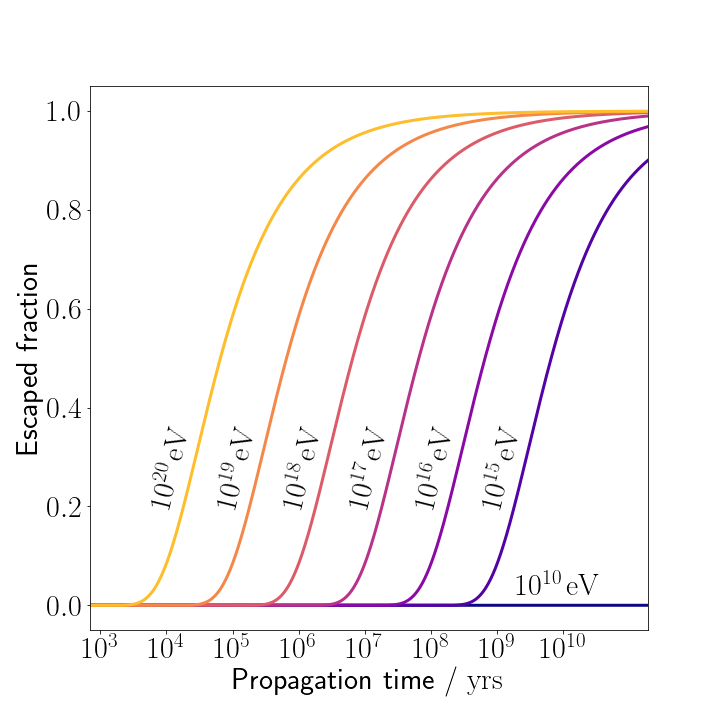
\includegraphics[width=\textwidth]{./plots/galactic_diffusion.png}
		\caption{\textbf{Escape fraction}}
		\label{fig:escape-fraction}
	\end{subfigure}
	\hfill
	\begin{subfigure}[b]{0.68\textwidth}
		\centering
		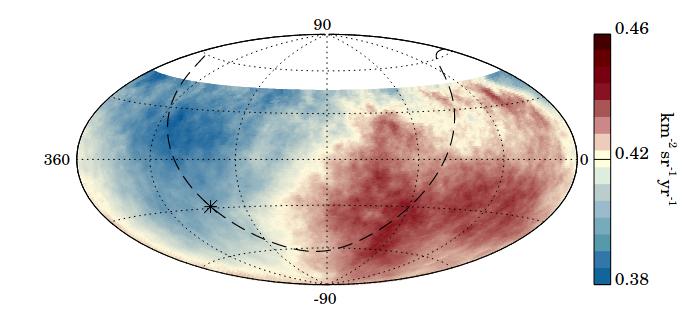
\includegraphics[width=\textwidth]{./plots/auger_dipole.png}
		\caption{\textbf{AD anisotropy}}
		\label{fig:ad-anisotropy}
	\end{subfigure}
	\caption{\textbf{(a)} $r_\text{esc.}(t)$ according to \autoref{eq:escape-fraction} for protons of different energies.\\ \textbf{(b)} Dipole in the arrival
	direction of CRs with $E>\SI{8}{\exa\electronvolt}$. Image copied from \cite{pierre2017observation}.}
\end{figure}

It can quickly be verified that a solution to the transport equation in this case is given by a normal distribution with mean $\upmu = 0$ and standard deviation 
$\sigma = \sqrt{2D_zt}$. The diffusion coefficient $D_z$ is a measure of how quickly the population spreads out (along the $\pm z$-direction). According to 
\cite{skilling1970diffusion}, $D_z$ can be parametrized via the particles energy $E_p$, and characteristics of the present $\vec{B}$-fields.

\begin{equation}
	\label{eq:diffusion-coefficient}
	D_z =\frac{1}{3}\,\frac{E_p}{m_p\,c^2}\cdot\frac{|\vec{B}|\cdot\langle L_{\vec{B}}\rangle}{\sqrt{\upmu_0\,\rho_\text{ISM}}},
\end{equation}

where $\langle L_{\vec{B}} \rangle$ is the characteristic length scale of deflecting $\vec{B}$-fields, $\upmu_0$ and $\rho_\text{ISM}$ are the magnetic vacuum 
permeability and density of the interstellar medium respectively. After some time $t$, a fraction $r_\text{esc.}(t)$ of particles will have a $z$-coordinate 
$|z| > H$, and exit the disc consequently. In reality, this is not equivalent to the particle leaving the galaxy, as large-scale halo structures extend above and 
below the visible disc \cite{searle1978compositions}. These halos are ignored here. $r_\text{esc.}(t)$ can thus be calculated according to 
\autoref{eq:escape-fraction}. For some selected energies, a plot of the escaping ratio over time is offered in \autoref{fig:escape-fraction}.

\begin{equation}
\label{eq:escape-fraction}
r_\text{esc.}(t) := 1 - \int\limits_{-H}^{H} \frac{n(z,t)}{n_0}\,\text{d}z
\end{equation}


It can be concluded that low energy CRs do not travel outside their host galaxy within reasonable timeframes. Meanwhile UHECRs with energies exceeding 
$E>10^{18}\,\text{eV}$ escape swiftly on ballistic trajectories and are thus likely have an extragalactic origin, not last also due to the limited energies that CR
sources in the milky way can provide.

This observation is consistent with a dipole in the \textbf{A}rrival \textbf{D}irection (AD) of UHECRs observed by the Pierre Auger observatory. The dipole points
roughly in the opposite direction of the galactic core, marked with an asterisk in \autoref{fig:ad-anisotropy}.

\subsection{Extragalactic propagation \& GZK-Cutoff}
\label{ssec:gzk-cutoff}

In the last paragraph the (likely) extragalactic origin of UHECRs was discussed. Such particles must traverse millions of lightyears of extragalactic space before
inducing a large air shower on earth. As the energy of these primaries increases above the \textbf{G}reisen-\textbf{Z}atsepin-\textbf{K}usmin threshold (GZK),
their propagation through space is thought to be severely impeded. At energies above $\approx10^{20}\,\text{eV}$ the \textbf{C}osmic \textbf{M}icrowave
\textbf{B}ackground (CMB) consisting of photons in the microwave range are blueshifted to energies $E_\gamma > \SI{300}{\mega\electronvolt}$. A proton with the 
corresponding energy can thus absorb such CMB photons and convert to its' excited spin state, the $\Delta^+$-baryon. The $\Delta^+$-baryon decays nearly 
instantanouely to (for example) the ground state again, by radiating away a $\pi^0$ and losing energy in the process \cite{PDG}. 

The mean free path of this interaction, also labelled GZK horizon is both energy- and primary-dependant. For \SI{75}{\exa\electronvolt} protons, it is 
$\approx \SI{100}{\mega\parsec}$ \cite{greisen1966end}. Cosmic rays exceeding the GZK threshold should ergo not be observed from faraway sources, and an overall 
reduction in flux at these energies should be recorded \cite{zatsepin1966j}.

Indeed, results published by the Auger collaboration (see \autoref{sec:cr-energy-spectrum}) are consistent with this assumption. Whether or not the GZK-supression
is the main cause for this soft spectrum at the highest energies remains unclear for now, but might be answered with the ongoing 
AugerPrime upgrade of the Pierre Auger observatory. 

\section{Composition}
\label{sec:cr-composition}

The composition of CRs largely mirror the relative abundancies of elements in the universe with some noteable exceptions shown in \autoref{fig:cr-composition}.
Elements like beryllium (Be) or vanadium (V) are atypical products of supernovae and thus not as common as e.g. oxygen (O) \cite{gamezo2005three, cowan2004r} in
the solar system. This leads to a dip in the corresponding abundancy spectrum. The same dip is not observed in CR primary abundancies. While it is a priori 
existant upon creation of cosmic rays, it gradually gets "filled up" via e.g. spallation processes during their propagation until an equilibrium state is reached.

This equilibrium state depends sensitively on the characteristic age of cosmic rays, i.e. the mean travel time until a particle escapes the galaxy. Measuring CR 
composition hence enables the estimation of this parameter. Such an analysis is conducted in \cite{garcia1977age}, where it is found that the observed abundancies 
are consistent with a characteristic age of \SI{1.7e7}{\year} for such high energy particles.

Contrary, hydrogen (H) and helium (He) are underrepresented (w.r.t their natural abundancy in the solar system) in cosmic ray particles. This is likely due to the 
comparably high ionization energy of both elements, which leads to less readily available hydrogen/helium ions. Since the acceleration mechanisms discussed in 
\autoref{sec:cr-acceleration} all couple to the net charge $q$ of a particle, unionized hydrogen and helium are not accelerated \cite{wang2002measurement}.

\begin{figure}
	\centering
	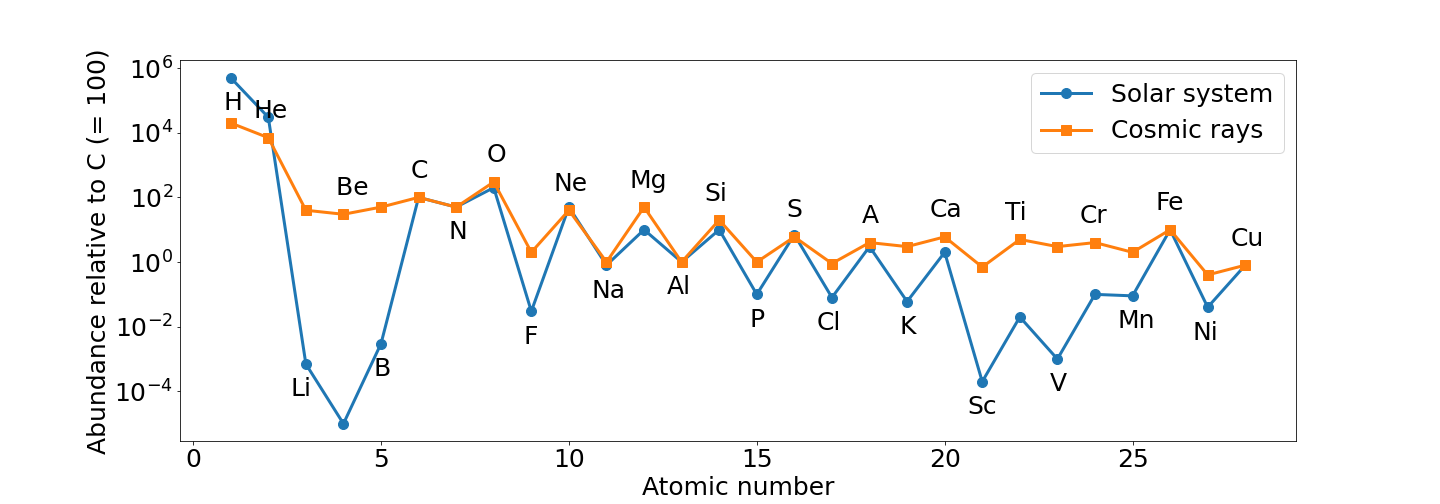
\includegraphics[width=1\textwidth]{./plots/cosmic_ray_composition.png}
	\caption{Composition expressed as abundancy relative to carbon for different sources. The ragged, alternating structure stems from an increased stability of 
	nuclei with an even amount of protons (c.f. for example \cite{kirson2008mutual}). Data from \cite{gaisser2016cosmic}}
	\label{fig:cr-composition}
\end{figure}

\section{Energy spectrum}
\label{sec:cr-energy-spectrum}

\begin{figure}
	\centering
	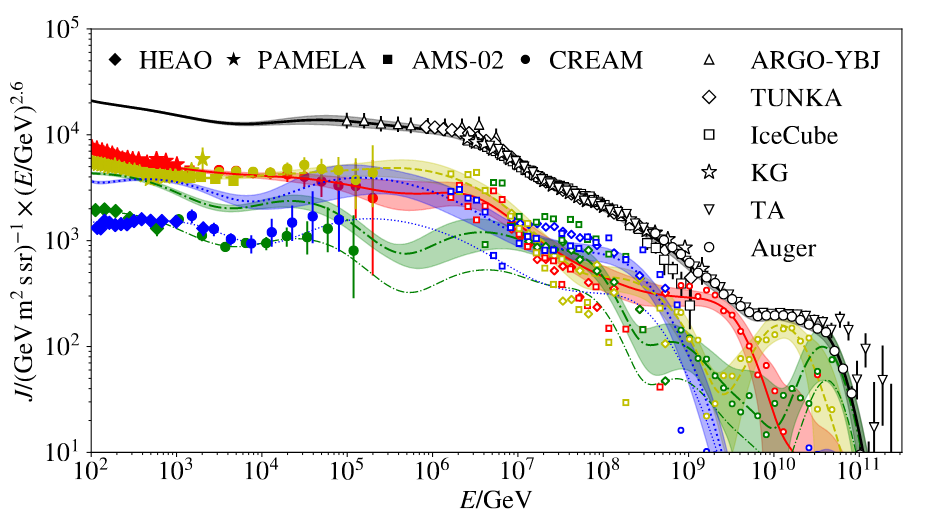
\includegraphics[width=1\textwidth]{./plots/cosmic_ray_spectrum.png}
	\caption{Measurements of the cosmic ray flux, multiplied by a factor $E^{2.6}$ for all types (black), and broken down by primary. Shown are protons (red), 
	helium (yellow), oxygen (green) and iron (blue). Plot adopted from \cite{dembinski2017data}.}
	\label{fig:cr-energy-spectrum}
\end{figure}

It has been discussed in \autoref{sec:cr-acceleration} that the expected CR flux w.r.t energy for supernova remnants is a powerlaw in the rough range of 
$\SI{200}{\mega\electronvolt} < E \lesssim \SI{100}{\tera\electronvolt}$. Observations by various experiments extend this result to even higher energies. Their 
combined results are shown in \autoref{fig:cr-energy-spectrum}. However, while the general assumption of a powerlaw $\Upphi(E)\propto E^\alpha$ holds over a large
range of energies, kinks and other feature in the spectrum indicate that the spectral index $\alpha$ is not uniform, and instead a function of energy. The 
approximate form of $\alpha(E)$ will be discussed in the following by examining several key regions of the energy spectrum. 

\TODO{reformat this in some better way}

\subsection{The proton knee; $\alpha(E < 10^{15}\,\SI{}{\electronvolt}) = 2.7 \rightarrow \alpha(E > 10^{15}\,\SI{}{\electronvolt}) = 3.0$}
\label{ssec:cr-proton-knee}

Below an energy of $\approx \SI{1}{\peta\electronvolt} = 10^6\,\SI{}{\giga\electronvolt}$, it is $\alpha(E)\approx 2.7$, while above a spectral index of 
$\alpha(E)\approx 3.0$ is found \cite{gaisser2016cosmic}. This softening of the spectrum (i.e. fewer particles of higher energy) could be attributed to several
effects.

\begin{itemize}
	\item \textbf{Dark matter channel} (partially falsified)

	\textbf{W}eakly \textbf{I}nteractive \textbf{M}assive \textbf{P}articles (WIMPs) are a popular candidate for \textbf{D}ark \textbf{M}atter (DM), as they 
	correctly estimate the cosmological evolution of the universe \cite{klypin1993structure}. A WIMP with a sufficiently high mass could explain the kink in the 
	energy spectrum. CRs with $E > m_\text{WIMP}c^2$ could in theory produce DM in deeply-inelastic scattering processes. The degree of steepening in the spectrum 
	is a measure for how readily the process $X \rightarrow \text{WIMP} + Y$ occurs. The steeper the spectrum gets, the more particles are converted to DM, and the
	higher the corresponding cross sections are. Most theories involving WIMP creation can be excluded, since detectors at earthbound particle accelerators should 
	have observed DM production at the observed steepening from $2.7$ to $3.0$ \cite{donato2009constraints}.

	\item \textbf{Escape during propagation}

	While the analysis in \autoref{ssec:transport-equation} concludes that the escape time for $\,10^{15}\,\text{eV}$ protons to leave their host 	galaxy is at 
	least of the order ${10^{8}}\,\text{yr}$ (compare \autoref{fig:escape-fraction}), the calculations leading to this result are extremely simplified. If a more 
	accurate treatment finds that particles with rigidities corresponding to the relevant energies are no longer confined by galactic magnetic fields, the kink 
	could originate from particles leaving the milky way and not contributing to the flux observed on earth any longer.

	\item \textbf{Limited source energy}

	A last possible explanation might lie in \autoref{eq:hillas-formula}. A prevalent acceleration mechanism for CRs below $10^{15}\SI{}{\electronvolt}$, such as 
	shock acceleration in SNRs for example, might not be able to provide energies exceeding this threshold due to physical constraints. The spectrum above the 
	proton knee is thus populated by CRs that originate from different acceleration mechanisms with differen relations $\alpha(E)$.
\end{itemize}

\subsection{The iron knee; $\alpha(E < 10^{17}\,\SI{}{\electronvolt}) = 3.0 \rightarrow \alpha(E > 10^{17}\,\SI{}{\electronvolt}) = 3.0$}
\label{ssec:cr-iron-knee}

The spectrum exhibits various similar kinks at slightly higher energies than the one discussed in \autoref{ssec:cr-proton-knee}, while it is assumed that they are 
ultimately caused by the same physical principles, each one corresponds to a different primary particle. Representatively, the iron knee at 
$E \approx 10^{17}\,\text{eV}$ is discussed here. 

Because iron has both a higher mass and charge ($Z = 26$, $A = 56$) compared to the proton ($Z = A = 1$), different processes couple to the different nuclei with 
disparate strength. In particular, an iron core has a higher magnetic rigidity $R \propto \frac{A}{Z}$ than a proton of equivalent energy. This is explained by the
fact that, while the iron core experiences a larger Lorentz force ($\propto Z$), the resulting acceleration ($\propto \frac{Z}{A}$) is not as strong due to a
disproportionally larger mass ($\propto A$). It is thus logical to expect differences in the creation, propagation, and shower characteristics 
(see \autoref{ssec:superposition-principle} for details) of different CR primary particles. By extension, the spectral index $\alpha(E)$ should be contrasting for 
each distinct particle type $i$, giving rise to different fluxes $\Upphi(E)_i$, which is confirmed by \autoref{fig:cr-energy-spectrum}.

The ultimate cause of the different knees remains unknown currently. In the context of the ongoing AugerPrime upgrade, the Pierre Auger observatory will scan the
energy spectrum at higher precision \cite{castellina2019augerprime}. This will allow to test whether the location of the various kinks scale with $A$ or with $Z$, 
and consequently shed light on the processes giving rise to these features.

\subsection{The Ankle $E \approx 10^{18}\,\SI{}{\electronvolt}$}
\label{ssec:cr-ankle}

At an energy of roughly $\approx\SI{1}{\exa\electronvolt} = 10^9\,\SI{}{\giga\electronvolt}$ an inflection point is found, where the spectrum hardens again from an 
index $\alpha(E) = 3.0$ to $\approx 2.7$. This might mark the final transition from predominantely galactic to intergalactic cosmic rays. If intergalactic CR 
sources such as AGNs have a harder spectrum (but lower luminosity) than galactic sources, the ankle could be well explained by a smooth transition from the latter to 
the former spectrum \cite{aloisio2007dip}. Other explanations focus on a change of the primary composition, which seems to be apparent in 
\autoref{fig:cr-energy-spectrum} at the correct energy \cite{allard2012extragalactic}. In any case, more data needs to be gathered to come to an informed 
conclusion on the ultimate cause.

\subsection{The suppression $E \approx 10^{20}\,\SI{}{\electronvolt}$}
\label{ssec:cr-cutoff}

At energies beyond $10^{20}\,\text{eV}$ a sharp drop in the flux can be noted. This represents the tail end of the spectrum, beyond which events are so rare that 
cosmic ray observatories can mostly just identify upper limits with their available statistics. The cause for the drop is actively debated, and might lie in the 
GZK cutoff discussed in \autoref{ssec:gzk-cutoff}. Another explanation might be that the tail end represents the point at which even the largest and most powerful
(in terms of energy) CR sources in the universe are not able to accelerate particles any further (c.f. \autoref{fig:hillas-plot}). 